% !TeX root = ../msc_thesis_jayd.tex
\chapter{Active Media and Radiation}
The previous chapter set the stage for the study of 
the scattering of light on general, albeit passive, 
potentials. The relative simplicity of the geometry
and of the physics allowed for a solution rich 
in physical information and lead to a rather simple
numerical solution. 

In the first section, we test the limits of the our analytical formalism
and of our numerical advances. To more accurately model
microlasers, we model the interaction of light with the underlying
quantum gain medium, i.e. we solve the Maxwell-Bloch, or Schrödinger-Bloch, 
matter equations. We will specifically use the \gls{salt}, a recently 
formulated steady state laser theory. In this theory, the effect 
of the active medium is reduced to an additional frequency and pump-dependent
term in the refractive index. This extra term has a Lorentzian frequency
dependence, as physically expected, and has non-zero real and imaginary
parts. The fragility of our extension of SQA is then exposed and some replacement
methods are suggested. 


The second section studies the experimental response
of different realizations of a specific type of antenna
known as \glspl{lcx}. The genesis of this study lies in
the hopes of designing an antenna that can be seamlessly
integrated into textile. The sheer complexity of the
antenna, as we will show, bars the use of the methods developed
in this essay in favour of the all-numerical \gls{fem}. 
This particular choice will be motivated and the design 
parameters of the antenna thoroughly explained. 

\section{Lasing and Scattering}
A recently formulated laser theory, named the 
\gls{salt} and developed by A. D. Stone's group
at Yale, has been shown to be an accurate model 
of the light-matter interaction involved in bidimensional
microlasers. Its steady-state nature allows us to apply
the formalism developed in the previous section 
to the theory. However, in light of the several shortcomings
of the \gls{sqa}'s numerical implementation, we have studied 
two other numerical methods. The first one, the \gls{vpm}, is based on 
differential equations and shares some of the problems of 
the onion method, but has a nice physical interpretation
in terms of phases and is more easily generalizable to 
3D scattering. 
To find a more robust solution, we completely forgo 
differential equations in favour of integral ones. 
Our brief incursion into the rich field of integral equations
is a rather recent one, and might leave the reader hungry for more.

\subsection{Primer on Steady State ab initio Laser Theory (SALT)}
Our exposition of \gls{salt} will be divided into two main sections:
the first will describe the details of the interaction of light with
the quantum gain medium and provide a steady-state solution
of the resulting Maxwell-Bloch equations. The second
will discuss the constant-flux states and their computation
using the aforementioned numerical methods. 

\paragraph{Solving the Matter Equations}
Our starting point, as always, is
  \begin{align}
   \nabla\times\bo{E}	&= ik\mu\bo{H};	&	\nabla\times\bo{H}	&= -ik\epsilon\bo{E}-ik\bo{P}^{NL}
  \end{align}
where $\bo{P}^{NL}$ now represents the possibly non-linear response
of the underlying quantum gain medium to the electric field $\bo{E}$.
We separate the fields in transverse and longitudinal
components, as we did for the passive cavities. Assuming 
that the propagation constant $\beta$ vanishes, we can 
separate two polarization states and write decoupled differential
equations for the longitudinal components of the fields
	\begin{subequations}
	\begin{align}
		\left[\nabla^2+k^2n^2\right]E_z	&= \frac{1}{\mu}\nabla E_z\cdot\nabla\mu -k^2\mu P_z	\tag{\theequation.TM}\\
		\left[\nabla^2+k^2n^2\right]H_z	&= \frac{1}{\epsilon}\nabla H_z\cdot\nabla\epsilon-
											\frac{ik}{\epsilon}\bo{P}^{NL}\times\nabla\epsilon
											-ik\nabla\times\bo{P}^{NL}							\tag{\theequation.TE}\label{eq:active.salt.TEeqn}
	\end{align}
	\end{subequations}
where the last equation is the \textit{proper} generalization for TE modes. 
To derive these equations, we made the implicit assumptions that the 
non-linear electric susceptibility tensor, 
	\begin{equation}
		\bo{P}^{NL} = \bo{\chi_e}^{NL}(\bo{r};\omega)\bo{E}(\bo{r}),
	\end{equation}
is at least a diagonal tensor, or a scalar. In the TM polarization, 
$E_r=E_\theta=0\Rightarrow P_r=P_\theta=0$, such that $\bo{P}^{NL}$
has a single non-zero component, while in the TE polarization only
the $P_r$ and $P_\theta$ components are non-zero. The vectors resulting
from the cross-product and curl in \eqref{eq:active.salt.TEeqn} possess
only a $z$-component, as needed. 

To go any further, we must compute the value of the non-linear electric
susceptibility tensor. 
To show the main features of the theory, we assume a two-level quantum 
system as the gain medium, although the method is generalizable to 
multi-level systems \cite[\S2.3]{GE2010b}. 

\begin{figure}
 \begin{center}
 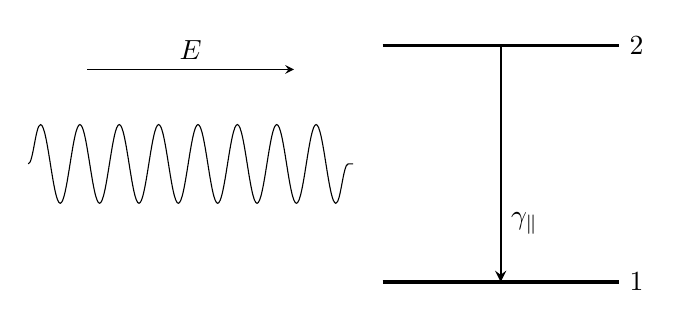
\begin{tikzpicture}[scale=1.5]
  % -- Draw quantum system. 
  \draw[very thick] (0,0) -- (2,0) node[right] {$\Ket{1}$};
  \draw[very thick] (0,2) -- (2,2) node[right] {$\Ket{2}$};
  \draw[thick,->,>=stealth] (1,2) -- (1,0) node[near end,right] {$\gamma_\parallel$};
  
  % -- Draw incoming light.
  \draw[decorate,decoration={snake,amplitude=0.5cm,segment length=0.5cm}] (-3,1) -- (-0.25,1);
  \draw[->,>=stealth] (-2.5,1.8) -- (-.75,1.8) node[midway,above] {$\bo{E}$};
 \end{tikzpicture}
 \end{center}
 \caption[Pictorial representation of the quantum gain medium]
	 {Pictorial representation of the interaction between the
	 quantum gain medium and the incoming field. The quantum system has 
	 two levels, the wavefunction being either $\Ket{1}$ or $\Ket{2}$. The relaxation
	 rate from level 2 to level 1 is given by $1/\Gamma_{21}$.}
 \label{fig:active.salt.twoLevelSystem}
\end{figure}

Solving Schrödinger's equation for a ``bare'', i.e. non-interacting
two-level system yields
  \begin{equation}
   H_0\Ket{\psi}=\omega_j\Ket{\psi}	\qquad j=0,1
  \end{equation}
and corresponding eigenfunctions $\Ket{1}$ and $\Ket{2}$. 
The incoming light field acts as a perturbation and source of energy
that stimulates a population transfer from level 1 to level 2 that decay
at rate $1/\gamma_\parallel$. The perturbation can be written as
  \begin{equation}
   H_1 = e\bo{\mu}\cdot\bo{E}
  \end{equation}
where $e$ is the electric charge and $\bo{\mu}$ is the 
dipole moment tensor of the material.  We expand the solution 
of the perturbed in the states of the unperturbed system
  \begin{equation}
   \Ket{\psi_1(t)}=C_1(t)\Ket{1}+C_2(t)\Ket{2}
  \end{equation}
and form the density matrix
  \begin{equation}
   \rho(t) = \Ket{\psi_1(t)}\Bra{\psi_1(t)}.
  \end{equation}
It allows us to solve the problem for an ensemble
of two-level systems \cite{GE2010b}.
Using the well-known evolution equations of the density
matrix \cite[\S6.2]{BOY2008} and defining
$D=\rho_{22}-\rho_{11}$, the population difference between the two
levels,  we obtain the equations
\cite[\S5.3]{HAK1985b}
  \begin{align}
   \dot{\bo{P}}^{NL}	&= -\left(i\omega+\gamma_\perp\right)\bo{P}^{NL}+\frac{g^2}{i\hbar}\bo{E}D	\\
   \dot{D}				&= \gamma_\parallel\left(D_0-D\right)-\frac{2}{i\hbar}\bo{E}\cdot\bo{P}^{NL}
  \end{align}
where $g^2$ is the dipole moment of the system, 
$\gamma_\perp$ is an \textit{ad hoc} phenomenological damping
term that comes from the interaction of the ensemble of systems\footnote{The author surmises that it 
could be computed with a mean field approximation.}
and $D_0$ is the equilibrium population. The approach 
uses a \gls{rwa}, but, contrary 
to most derivations, does not invoke the \gls{svea}. 
One of the main approximations, one that is necessary to make
ground, is the \gls{sia}, i.e. $\dot{D}=0$. Writing the fields
as Fourier series
	\begin{align*}
		\bo{P}^{NL}	&= \sum_{\mu}\bo{p}_\mu e^{-ik_\mu t}	&	\bo{E}	&= \sum_{\mu} \bo{\Psi}_\mu e^{-ik_\mu t}
	\end{align*}
leads to the relationship\footnote{We have skipped some steps. See \cite[\S2.2]{GE2010b} for details.}
  \begin{equation}
   \bo{p}_\mu = \frac{g^2}{\hbar}\frac{1}{k_\mu-k+i\gamma_\perp}\frac{D(\bo{r})}{1+\sum\frac{4g^2}{\gamma_\perp\gamma_\parallel}\Gamma(k_\mu)\left|\Psi_\mu(\bo{r})\right|^2}\bo{\Psi}_\mu(\bo{r}).
  \end{equation}
In the TM polarization, this leads to the equation
  \begin{equation}
   \left[\nabla^2+k^2\left(\epsilon(\bo{r})+\frac{g^2}{\hbar}\frac{1}{k_\mu-k+i\gamma_\perp}\frac{D(\bo{r})}{1+\sum\frac{4g^2}{\gamma_\perp\gamma_\parallel\Gamma(k_\mu)}\left|\Psi_\mu(\bo{r})\right|^2}\right)\right]\Psi_\mu(\bo{r})=0
  \end{equation}
where
	\begin{equation}
		\Gamma(k_\mu) = \frac{\gamma_\perp^2}{(k-k_\mu)^2-\gamma_\perp^2}.
	\end{equation}

\paragraph{Constant-flux States and Scattering}

\todo[inline]{Detail non-Hermitian problem defined by CF states. Methods of solution 
to the possibly non-linear equations.}

\subsection{Methods of Solution}
\paragraph{Variable Phase Method}
This elegant method has its roots deep in the literature of quantum-mechanical
scattering. It is based on the fact that, for central potentials, the 
\gls{sMatrix} is diagonal and that its elements can be written as
$e^{i\delta_k}$, where $\delta_k$ is the phase shift suffered by the 
$k$th partial wave. One can thus find a first order, non-linear differential
equation \cite{CAL1967} for each $\delta_k$. The method transforms the \gls{bcp} to an \gls{ivp}, as the phase shift
is bounded. In our present case, the potential is not a central one and the
\gls{sMatrix} is not diagonal. We will need to solve a coupled system 
of differential equations to represent the coupling between the different
partial waves. The \gls{vpm} will give rise to an \gls{ivp} matrix \gls{ode}.

The initial motivation for the use of \gls{vpm} was the computation 
of the field inside the scatterer. In the \gls{sqa}, modifying 
the linear algebra operations of the reduction phase yields
an algorithm that computes the field from given $\bo{A}$ and $\bo{B}$
coefficients. It is unfortunately highly unstable, to the point 
of being unusable. The authors of \cite{FOR2012} suggested that
the \gls{vpm} was stable, suggesting its use over the onion
discretization of \gls{sqa}. While the \gls{vpm} has some inherent
issues and our implementation is far from complete, we present
here the main development both for the interested reader and for 
future reference. 

The method starts with the angular momentum expansions
  \begin{subequations}
  \begin{align}
   H_z(r,\theta)	&= \frac{1}{\sqrt{2\pi}}\sum_{m=-\infty}^\infty \frac{1}{\sqrt{r}}\psi_m(r)e^{im\theta}	\\
   n(r,\theta)		&= \frac{1}{\sqrt{2\pi}}\sum_{m'=-\infty}^\infty n_{m'}(r)e^{im'\theta}.
  \end{align}
  \end{subequations}
Substituting these expansions in Helmholtz's equation and projecting
onto the eigenstate $\sqrt{r}e^{-im''\theta}/\sqrt{2\pi}$ yields a
system of coupled \glspl{ode} for each moment of the field $\psi_m$
	\begin{equation}
		\label{eq:active.vpm.equation}
		\bo{\psi}''-\frac{\mat{M}^2-\mat{I}/4}{r^2}\bo{\psi}+\frac{k^2}{2\pi}\mat{N}^2\bo{\psi}=0
	\end{equation}
where 
	\begin{equation*}
		\left[\mat{N}(r)\right]_{mm''}=\sum_{m'}n_{m'}(r)\delta_{m+m',m''}.
	\end{equation*}
Notice that the free case is recovered when $n(r,\theta)=1$, as 
then $n_{m'}=\delta_{m'0}$ and 
	\begin{equation}
		\bo{\psi}''-\frac{\mat{M^2}-\mat{I}/4}{r^2}\bo{\psi}+k^2\bo{\psi}=0
	\end{equation}
a system of uncoupled Bessel equations. At this point, we 
introduce the matrix \gls{ode}, i.e. \eqref{eq:active.vpm.equation} with as many 
rows as columns. Each column solves the ODE, but has different boundary conditions
\cite[\S15.2]{NEW1982}. Since the scattering solution must obey Sommerfeld's radiation
condition, we use the factorization
	\begin{equation}
		\bo{\psi} = \mat{G}_k(r)\mat{W}^{+}(kr)
	\end{equation}
where $\left[\mat{W}^{\omega}(kr)\right]_{mm''}=H_m^{(\omega)}(kr)\delta_{mm''}$.
Outside the \gls{lss}, the solution must be $\mat{W}^+(kr)$. In the general potential
scattering theory, the \gls{lss} is usually a sphere at infinity, which yields the 
initial value conditions
	\begin{align}
		\mat{G}_k(\infty)	&=\mat{I}	&	\mat{G}_k'(\infty)=\mat{0}.
	\end{align}
with 
	\begin{equation}
		\mat{G}_k''+2\mat{G}_k'\frac{d\log\mat{W}^\omega}{dr}+\frac{1}{r^2}\left[\mat{G}_k,\mat{M}^2-\mat{I}/4\right]
					+\frac{k^2}{2\pi}\left(\mat{N}^2-2\pi\mat{I}\right)=0.
	\end{equation}

The $\mat{G}_k(r)$ matrix represents the phase shifts accumulated by each partial wave $m$ 
and caused by the $m'$th angular moment of the potential. The factorization procedure 
effectively transforms the \gls{bcp} to an \gls{ivp}, with the data provided on the 
\gls{lss}. The matrix ODE can thus be solved by using any good integration routine\footnote{Although
make sure you use a stiff equation solver. See Appendix \ref{sec:app.basisEqn.vpm} for details.}.

The scattering matrix of the problem can also be obtained if we 
compute the conjugate solution, solving with the incoming radiation $\bo{\psi}=\mat{G}_{-k}\mat{W}^-(kr)$
instead of the outgoing one. The physical wave function is thus given by 
	\begin{equation}
		\bo{\psi} = \mat{G}_{-k}(r)\mat{W}^-(kr)+\mat{G}_k(r)\mat{W}^+(kr)\mat{S}_k(k).
	\end{equation}
Using the finiteness condition of the field at origin, we have
	\begin{equation}
		\mat{S}_k = -\lim_{r\rightarrow0}\left(\mat{W}^{+}(kr)\right)^{-1}\mat{G}_k^{-1}(r)\mat{G}_{-k}(r)\mat{W}^-(kr).
	\end{equation}

\paragraph{Green's Function Method}
Seeing the differential methods fail, the author of this essay, 
then on the brink of despair, first took notice of the 
power of integral methods. Simply rewriting Helmholtz's 
equation as
  \begin{equation}
   \left[\nabla^2+\epsilon_B(\omega)k^2\right]\psi=-k^2\Delta\epsilon(\bo{r};\omega)\psi
  \end{equation}
where 
  \begin{equation}
  \Delta\epsilon(\bo{r};\omega)=\epsilon(\bo{r};\omega)-\epsilon_B(\omega)
  \end{equation}
where $\epsilon(\bo{r};\omega)$ is the permittivity profile of the scatterer
and $\epsilon_B(\omega)$ the constant permittivity of the environment, or background.
This allows to write a formal solution using the Green's function of Helmholtz's equation
  \begin{equation}
   \psi(\bo{r}) = \phi(\bo{r}) - k^2\mathop{\iint}_\mathcal{C}G(\bo{r},\bo{r}')\Delta\epsilon(\bo{r}';\omega)\psi(\bo{r}')d^2\bo{r}'
  \end{equation}
where $\phi(\bo{r})$ is a solution of the homogeneous problem and
  \begin{equation}
   G_\omega(\bo{r},\bo{r}') = -\frac{i}{4}H_0^{(\omega)}(k\sqrt{\epsilon_B}|\bo{r}-\bo{r}'|)
  \end{equation}
and we use the \textit{outgoing} Green's function $G=G_+$.

Instead of a \gls{pde}, we now must solve an implicit 
integral equation for the field. It is a Fredholm 
equation of the second kind with a weakly singular, compact
operator. This ensures the existence
and uniticity of the solution \cite{GOH1981,COL2013}.
We solve the surface integral equation in real space by meshing
the cavity $\mathcal{C}$. The details of the meshing is left to 
Appendix \ref{sec:app.basisEqn.greenFunction}. Let us denote the set
of cells of our mesh by $\Delta$. We can thus cast the integral
equation as
	\begin{equation}
		\psi_j = \phi_j -k^2\sum_{j'\in\Delta} G_{jj'}\Delta\epsilon_{j'}A_{j'}\psi_{j'}
	\end{equation}
where $\psi_j=\psi(\bo{r}_j)$ and similarly for the other quantities. We can
rewrite this as the matrix problem\footnote{This, of course, only holds if the
kernel is linear.} 
	\begin{equation}
		\left(\mat{I}+\mat{K}\right)\bo{\psi}=\bo{\phi}.
	\end{equation}
where 
	\begin{equation}
		K_{jj'} = G_{jj'}\Delta\epsilon_{j'}A_{j'}.
	\end{equation}

The matrix equation is then solved using any good 
linear algebra solver. This yields values for the
field inside the scatterer. The integral equation
is then explicit for the field outside the scatterer. 
Our interest, however, still lies in the computation
of the scattering matrix. It turns out that, if we
use 
	\begin{equation}
		\phi = J_M(kr)e^{iM\theta}
	\end{equation}
as the ``incoming'' field, one may find that the scattering
matrix can be computed via
	\begin{equation}
		S_{mM} = \delta_{mM} - \frac{ik^2}{2}\mathop{\iint}_\mathcal{C}e^{-im{\theta'}}J_m(kr')\Delta\epsilon(\bo{r}')\psi^{(M)}(\bo{r}')d^2\bo{r}'.
	\end{equation}
In Appendix \ref{sec:app.basisEqn.greenFunction}, we lay out the method in more detail, 
discuss the numerical implementation and present a generalization for the complete 
vectorial electromagnetic fields.

\subsection{Examples}

\section{Smart Textile Antennae}
The last part of this essay recounts the author's contributions
in a project involving the design and theoretical characterization
of fibre-antennas. This section departs a little from the more theoretical
and numerical musings of the others and presents both the modeling of the 
antennae and their experimental characterization.   

The goal of the original project was to develop an antenna that is compatible with 
WiFi standards (i.e. emits at $f=2.45\,\unit{GHz}$) and easily integrated
to textile. These two requirements impose multiple restrictions on both
the materials that can be used and the geometry of the antenna. For seamless
integration, we would like the antenna to be spun directly into the textile. 

Most solutions today merely affix a patch antenna to a less 
encumbered part of the textile \cite{CAT2004,JAI2013}, e.g. 
on the should pads of a shirt or the front of a t-shirt.
A metallic plate shields the user from the electronic components 
of the patch antenna. Because the properties of patch antennas are
well known \cite{ELL2003}, it requires very little engineering and is thus cheap. However, integration 
with the textile is far from seamless, as it is very apparent to the
user that he has become a giant walking antenna. Our project thus 
strives to find antenna designs that have emission properties
as flexible as a patch antenna's while improving textile integration
as to make it become transparent to the user.

The concept of a fibre-antenna rapidly established itself
as an ideal solution in the research group. It provides a rich
architecture upon which to build. Moreover, it can easily 
be spun into textile as it can loaded into the spools that 
deliver threads to looms. Its mechanical properties make it
fit for daily use as it can resist a trip in the washing machine. 
Integration of the electronic components inside that fibre 
serves to shield both the user and the components. 

Before showing the details of our contribution, 
we will first show the important quantities when
working with antennas, and more importantly the design
parameters.

\subsection{Basic Antenna Theory}
Even today, a full 140 years after the publication of 
Maxwell's \textit{Treatise on Electricity and Magnetism}, 
the electromagnetic modeling of radiating structures 
is an ongoing research problem. The notorious difficulty 
of solving Maxwell's equations seriously hampers analytical efforts
and, due to the nature of electromagnetic radiation, numerical
progress is not easier to achieve.

In what follows, we present the basic equations of 
antenna theory (Maxwell's) and discuss the nature 
of sources in this framework (currents and charges). 

\subsubsection{Maxwell's Equations}
Recall the macroscopic Maxwell equations in matter
\eqref{eq:passive.formalism.maxwellsEquations}, with the 
induced conduction current density given by
	\begin{equation}
		\bo{j}_c = \sigma\bo{E}.
	\end{equation}


A technical point is in order. In the antenna literature, the induced
currents and charge density are considered as the fundamental quantities 
that \textit{produce} the fields. While worthwhile (see the Stratton-Chu section), 
this viewpoint requires that either (i) we have \textit{a priori} knowledge of 
the sources ($\bo{J}_t=\bo{J}_c+\bo{J}_s$ and $\rho$) or (ii) that we use the
constitutive relations down the line. The first case applies to situations
where the induced current is trivially known (e.g. the dipole antenna) or
when $\sigma=0$ and $\bo{J}_s$ is known.

Also, even though the $\bo{H}$ field was introduced as an auxiliary field to take
into account the effect of an applied magnetic field to the material, we 
take it as the fundamental field as it leads to more easily solvable
equations and is a completely equivalent choice. 

\subsubsection{Stratton-Chu Solution}
In antenna problems, we want to compute the field values as a function of 
the sources that contribute to these fields. From electrostatics, we know 
that a current density $\bo{J}$ gives rise to an electric field and a charge 
density $\rho$ gives rise to a magnetic field. In the time-varying picture, 
the electric and magnetic fields become coupled and we take the viewpoint that
the $\bo{J}$ and $\rho$ give rise to both electric and magnetic fields. 

To compute the field from these sources, which are presupposed to exist, 
we must use the Stratton-Chu integrals. The derivation is standard, so we 
refer to \cite{ELL2003}. Consider a volume $V$ of free space containing
sources and possibly excluded sub-volumes $V_i$ bound by surfaces $S_i$ that contain matter
of some kind. By the use of Green's and Stokes' theorems and other vectorial 
identities, we find that the field outside the excluded sub-volumes
can be expressed as
  \begin{align}
   \bo{E} &= \frac{1}{4\pi}\mathop{\iiint}_V \left(\rho\nabla G+i\omega G\bo{J}\right)dV
	+\frac{1}{4\pi}\oiint_{S_1,\cdots,S_N}\left[\bo{n}\cdot\bo{E}\nabla G+(\bo{n}\times\bo{E})\times\nabla G+i\omega G(\bo{n}\times\bo{H})\right]dS\label{eq:active.antennae.strattonChuE}\\
   \bo{H} &= \frac{1}{4\pi}\mathop{\iiint}_V \bo{J}\times\nabla G dV
	+\frac{1}{4\pi}\oiint_{S_1,\cdots,S_N}\left[-i\omega G(\bo{n}\times\bo{E})+(\bo{n}\times\bo{H})\times\nabla G+(\bo{n}\cdot\bo{H})\nabla G\right]dS\label{eq:active.antennae.strattonChuH}
  \end{align}
where $G$ is the Green's function of the problem
  \begin{equation}
   G(\bo{r},\bo{r}') = \frac{e^{ik|\bo{r}-\bo{r'}|}}{4\pi|\bo{r}-\bo{r}'|}.
  \end{equation}

These two equations are rigorous solutions of Maxwell's equations. 
They can be used with any antenna and provide ways to compute the 
current distribution if is unknown (constitutes an integral equation in the current)
and can be used to compute the far-field of antennae when either 
(i) the current distribution is known or (ii) the near-field around the antenna
is known. 
These two properties discriminate antennae into two categories, denoted Type I and Type II.

Type I antennae have a well-approximated current distribution, which means that there are no
sub-volumes to be excluded and therefore no surface integrals in expressions 
\eqref{eq:antenna.strattonChuE} and \eqref{eq:antenna.strattonChuH}. 

On the other hand, Type II antennae have well-approximated near-fields, leading
us to exclude the volume containing the antenna. Expressions \eqref{eq:antenna.strattonChuE}
and \eqref{eq:antenna.strattonChuH} contain only surface integrals, then. 

\subsubsection{Antenna Parameters}
In the design of our antenna, we will want to optimize the value
of some parameters. We will now describe some of these parameters.

\paragraph[Directivity and Gain]{Directivity and Gain \cite[\S 1.16]{ELL2003}}
Given a radiation pattern measured (in the far-field) as the power density 
$\mathcal{P}(\theta,\varphi)$, we can define its \textit{directivity}
as
  \begin{equation}
   D(\theta,\varphi) = \frac{4\pi\mathcal{P}(\theta,\varphi)}
			{\int_0^\pi\int_0^{2\pi}\mathcal{P}(\theta',\varphi')\sin\theta'd\theta'd\varphi'}.
  \end{equation}
The value of the directivity is less than unity if the power density radiated at angle $(\theta,\varphi)$
is less than the average power radiated. For instance, an isotropic antenna will possess a unit directivity
for all angles while a highly directional antenna will have a sharp peak  in its directivity function 
at some angle $(\theta,\varphi)$.

Another interesting concept to introduce is \textit{partial directivity}. 
The power density can be divided into two contributions: the $\theta$-polarized
and the $\varphi$-polarized polarization and we can write
  \begin{equation}
    \mathcal{P}(\theta,\varphi) = \mathcal{P}_\theta(\theta,\varphi)+\mathcal{P}_\varphi(\theta,\varphi)
  \end{equation}
where the subscripts indicate the polarization state. The partial 
directivities hence follow
  \begin{equation}
   D(\theta,\varphi) = D_\theta(\theta,\varphi)+D_\varphi(\theta,\varphi).
  \end{equation}

We can also introduce the gain, which characterizes the loss
and the directivity of the antenna simultaneously. It is simply given
as
  \begin{equation}
    G(\theta,\varphi) = \frac{4\pi r^2\mathcal{P}(\theta,\varphi)}{P}
  \end{equation}
where $P$ is the power fed into the antenna. Because of the 
losses, 
	\begin{equation*}
		P/r^2>\int_0^\pi\int_0^{2\pi}\mathcal{P}(\theta',\varphi')\sin\theta'd\theta'd\varphi'
	\end{equation*}
such that $G(\theta,\varphi)<D(\theta,\varphi)$. 

We can also define partial gains in the exact same fashion we defined partial
directivities.

Radiation efficiency $\eta$ is defined as the ratio of the total radiated power 
to the power accepted by the antenna \cite{IEEE145-1993}.

\paragraph{Scattering Parameters}
The scattering parameters (or $S$-parameters) are
usually defined through a linear $N$-port network. 
Suppose we have an electronic device comprising
$N$ ports, or points of entry. Imagine shining light onto, 
or make a current flow into,
one of the ports, say port $j$. A certain percentage
of the power carried by this light be reflected 
by this port and the rest will be transmitted to the
other ports or absorbed in the medium. The \textit{reflection}
coefficient is given by $S_{jj}$ while the transmission
coefficients are given $S_{ji}$ ($i\neq j$) where $\mat{S}$
is the scattering matrix of the network. In a reciprocal (in the sense
of Lorentz) network, the scattering matrix will be equal to its
transpose, i.e. $S_{ij}=S_{ji}$. In a lossless network, the scattering
matrix will be unitary. 

This is, of course, highly reminiscent of the scattering operator
in quantum-mechanical scattering which relates the outgoing (scattered)
components to the incoming (incident) components
  \begin{equation}
   \Ket{\Psi_\text{out}}=\mathcal{S}\Ket{\Psi_\text{in}}.
  \end{equation}
In this case, the ``ports'' are the different angular momenta
components rather than physical input/output connections. 
The precise nature of ports is somewhat arbitrary in optical structures.

The traces of these parameters, i.e. the value of $S_{ij}$ as a function of 
the frequency of the input current, will be of primary interest. The frequency
response can give information about the finesse of the resonances, as well as
hinting at specific radiation mechanisms. The analysis below will be divided
in two parts: the analysis of the traces on their own, and comparison with the 
theoretical/simulation traces.

\subsection{The Leaky Coaxial Cable}
The modelization of \gls{lcx} is not a new field \cite{DEL1980,WAN2001,KIM2007,ADD2008}.
They have been studied using a variety of analytical and numerical methods. Most of them 
depend on a set of \textit{crucial} approximations that cannot be assumed to hold 
in our particular case.

\begin{description}
	\item [Periodicity of the structure] The $z$-periodicity of the geometry and 
		and material parameters paves the way for a Floquet-Bloch expansion of the 
		fields. This is used in \cite{WAN2001}.
	\item [Narrow slits] A perturbation theory, where slits are supposed to be 
			small as compared to the wavelength, $kS_z\ll1$, is used in \cite{KIM2007}.
	\item [Transmission line behaviour] One of the most important approximation, it stipulates
			that the \gls{lcx} supports a single TEM propagating mode. This allows the 
			unambiguous use of scalar voltages and currents as the physical observables
			\cite{PAU2007}. It also allows
			the use of simpler numerical methods, such as using the overlap between the 
			propagating mode and the radiation continuum to quantify the radiation 
			properties \cite{SHI1989,ADD2008}. 
\end{description}

In our case, the worst offender is the last one, as our metal deposition method
does not allow for a fine control of the thicknesses deposited, nor ensure its
smoothness. The TEM approximation relies on the metal layers behaving almost as 
perfect conductors. Our metallic layers are typically smaller than the skin
depth of the metal, which makes the approximation invalid. 

Moreover, we cannot consider the structure to be periodic, as the total 
length of the fibre-antenna is of the order of the wavelength ($\lambda\sim12\unit{cm}$) and the period
of the slots is smaller than the wavelength. Given the size of the slots, 
the author is comfortable to say that we neither are in the perturbation regime. 
Figure \ref{fig:antenna.fibre-antenna} shows the actual design and the important parameters.

\paragraph{Choice of simulation software}
Given the wild scale in the size of the structures (from the nanometer to the millimeter), we use
the FEM to solve the driven problem. The parameters of interest will be the scattering parameters, the
radiation pattern and antenna efficiency, gain and directivity. We will first model the fibre-antennae
that were fabricated. There will be a subsequent optimization phase.

\todo[inline]
{Discuss the passage from integral equations to finite element analysis.
Definition of transmission problem, other kinds of boundary conditions, all
difficult to account for in the traditional Fredholm form. Weak solution naturally
incorporates the boundary conditions and, while it has some issues, is more
easily solved.}

%As finite element methods directly solve Maxwell's equations, 
%they can be a useful tool to verify semi-analytical methods. 
%In the last section, we reported some agreement issues 
%between experimental and simulation data. We purported
%that the discrepancy was due to the small size of the
%silver layers that we could properly account for in 
%the finite element model. This issue has been solved
%by abandoning the idea of properly meshing the silver layers
%and replacing them by appropriate impedance boundary conditions.
%From HFSS's documentation, we see that the ``Layered Impedance 
%Boundary Conditions'' module follows the theory set forth in 
%\cite{MIT1968} and others. 

\begin{figure}
  \centering
  \begin{subfigure}[b]{\textwidth}
    \centering
   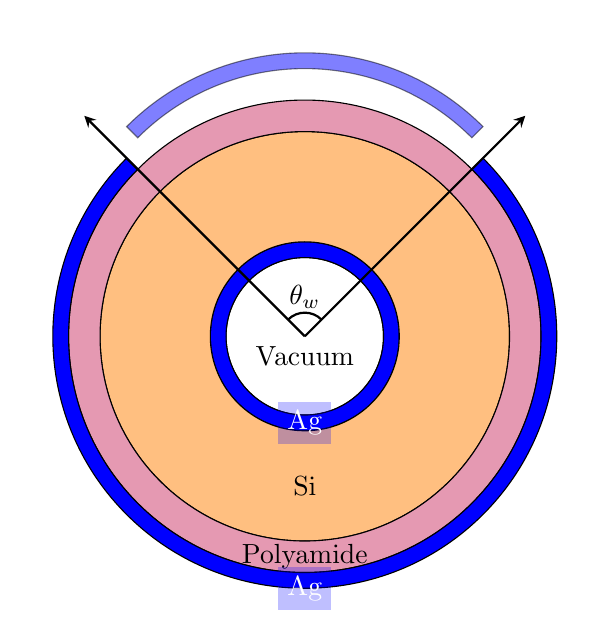
\begin{tikzpicture}
    % -- Draw different materials of the antenna.
    \coordinate (O) at (0,0);
    \draw (O) circle (1);											% Vacuum core
    \draw[fill=blue, even odd rule] (O) circle (1.2) (0:1) arc (0:360:1);					% Silver layer
    \draw[fill=orange!50!white, even odd rule] (O) circle (2.6) (0:1.2) arc (0:360:1.2);			% Dielectric (Si) layer
    \draw[fill=purple!40!white, even odd rule] (O) circle (3) (0:2.6) arc (0:360:2.6);				% Dielectric (polyamide) layer
    \draw[fill=blue,even odd rule] (45:3) -- (45:3.2) arc (45:-225:3.2) -- (-225:3) arc (-225:45:3) -- cycle;	% Second silver layer
    \draw[fill=blue,opacity=0.5,even odd rule,yshift=0.4cm] (45:3) -- (45:3.2) arc (45:135:3.2) -- (135:3) arc (135:45:3) -- cycle;
    
    % -- Draw the angular size of the window.
    \draw[->,>=stealth,thick] (O) -- (-2.8,2.8);
    \draw[->,>=stealth,thick] (O) -- (2.8,2.8);
    \draw[thick] (45:0.3) arc (45:135:.3); 
    \node at (0,0.5) {$\theta_w$};
    
    % -- Place text for materials
    \node at (0,-0.25) {Vacuum};
    \node[text=white,fill=blue,fill opacity=0.25,text opacity=1] at (0,-1.1) {Ag};
    \node at (0,-1.9) {Si};
    \node at (0,-2.8) {Polyamide};
    \node[text=white,fill=blue,fill opacity=0.25,text opacity=1] at (0,-3.2) {Ag};
   \end{tikzpicture}
   \vspace{0.25cm}
   \caption{View of the cross-section: in order of increasing radius, we have: vacuum, silver, silica, polyamide and silver.
	    We have shown a cross-section where there is a ``window''. When there are no windows, 
	    the outer silver layer takes up the entire circumference of the fiber.
	    $\theta_w$ is the angular size of the windows.}
   \label{fig:active.antennae.fibre-antenna.xsection}
  \end{subfigure}
  
  \vspace{4cm}
  
  \begin{subfigure}[b]{\textwidth}
    \centering
   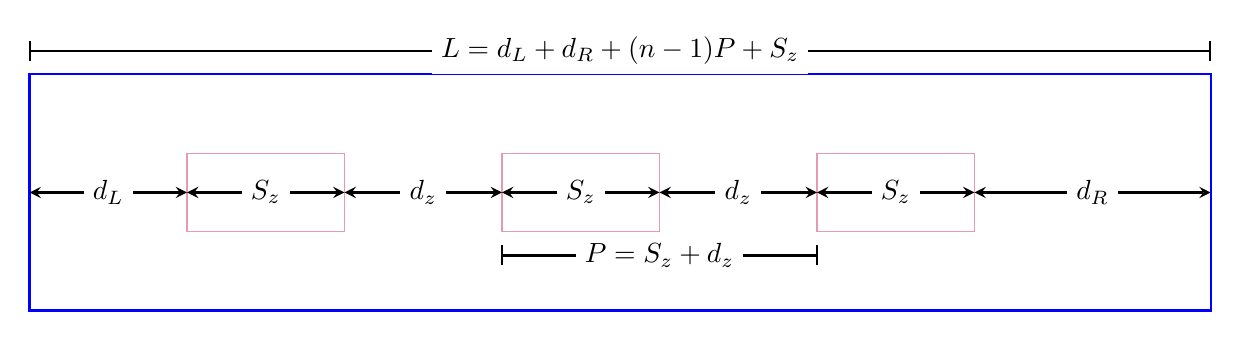
\begin{tikzpicture}
    \draw[blue,thick] (0,-0.5) rectangle (15,2.5);
    \draw[purple!40!white] (2,0.5) rectangle (4,1.5);
    \draw[purple!40!white] (6,0.5) rectangle (8,1.5);
    \draw[purple!40!white] (10,0.5) rectangle (12,1.5);
    
    \draw[<->,>=stealth,thick] (0,1) -- (2,1) node[midway,fill=white] {$d_L$};
    \draw[<->,>=stealth,thick] (2,1) -- (4,1) node[midway,fill=white] {$S_z$};
    \draw[<->,>=stealth,thick] (4,1) -- (6,1) node[midway,fill=white] {$d_z$};
    \draw[<->,>=stealth,thick] (6,1) -- (8,1) node[midway,fill=white] {$S_z$};
    \draw[<->,>=stealth,thick] (8,1) -- (10,1) node[midway,fill=white] {$d_z$};
    \draw[<->,>=stealth,thick] (10,1) -- (12,1) node[midway,fill=white] {$S_z$};
    \draw[<->,>=stealth,thick] (12,1) -- (15,1) node[midway,fill=white] {$d_R$};
    \draw[|-|,thick] (-0.01,2.8) -- (15.01,2.8) node[midway,fill=white] {$L=d_L+d_R+(n-1)P+S_z$};
    \draw[|-|,thick] (5.99,0.2) -- (10.01,0.2) node[midway,fill=white] {$P=S_z+d_z$};
   \end{tikzpicture}
   \vspace{0.25cm}
   \caption{Top view: the positions of the windows are usually asymmetric, i.e. $d_L\neq d_R$. The distance between
	    the windows is given by $d_z$ and the length of the windows are $S_z$. We notice that the length of the 
	    fibre is given by $L=d_L+d_R+(n-1)P+S_z$ where $P=S_z+d_z$ is the period between windows and $n$ is the number
	    of windows.}
   \label{fig:active.antennae.fibre-antenna.topview}
  \end{subfigure}
  \caption{Geometry of the fibre-antenna}
  \label{fig:active.antennae.fibre-antenna}
\end{figure}

\paragraph{Specifications of the Devices}
An image is worth a thousand words. Figure \ref{fig:antenna.fibre-antenna.xsection}
shows a cross-section of the fibre. Figure \ref{fig:antenna.fibre-antenna.topview} 
shows a top view of the antenna and display the positions of the windows. 
Multiple designs have been fabricated, but we retain only those that 
we have tried to simulate. Table \ref{tab:antenna.rfxx-parameters} 
shows the actual geometrical parameters of the fibre-antennas.

\subparagraph{On the thickness of the silver shells}
The thicknesses of the dielectric materials are provided by the manufacturer, 
Polymicro Technologies, safe for the thicknesses of the silver layers. 
For the time being, we have calculated those thicknesses by measuring
the DC resistance of the inner and outer layers of silver and
using the relation \cite[p.~204]{CHE1989}
  \begin{equation}
    \label{eq:active.antennae.dcResistivity}
    R = \frac{L}{\sigma A}
  \end{equation}
where $L$ is the length of the fibre, $\sigma$ the conductivity of the silver
layer and $A$ its area. For the inner and outer layers, we have
  \begin{align}
    A_\text{inner}	&= \int_0^{2\pi}\int_{t_\text{vac}-t_\text{Ag1}}^{t_\text{vac}}r\,dr d\theta= \pi\left(2t_\text{vac}t_\text{Ag1}-t_\text{Ag1}^2\right)	\\
    A_\text{outer}	&= \int_0^{2\pi}\int_T^{T+t_\text{Ag2}}r\,dr d\theta = \pi\left(2Tt_\text{Ag2}+t_\text{Ag2}^2\right)
  \end{align}
where $T=t_\text{vac}+t_\text{Ag1}+t_\text{Si}+t_\text{pyamide}$. 
Substituting these results into \eqref{eq:antenna.dcResistivity}
yields
  \begin{subequations}
  \label{eq:active.antennae.thickGeneralEquations}
  \begin{align}  
   -t_\text{Ag1}^2 + 2t_\text{vac}t_\text{Ag1}-\frac{L}{\sigma_\text{Ag0}\pi R_\text{inner}}	&=0	\\
   t_\text{Ag2}^2 + 2Tt_\text{Ag2}-\frac{L}{\sigma_\text{Ag0}\pi R_\text{outer}}			&=0
  \end{align}
  \end{subequations}
where the $R$s are the measured D.C. resistances for each shell. 
This can readily be solved using the quadratic equation. Using the bulk conductivity
of silver (see Table \ref{tab:antenna.physicalParameters}) yields the 
thicknesses found in Table \ref{tab:antenna.rfxx-parameters}.

\begin{figure}
 \begin{center}
 \begin{tikzpicture}
  % -- Draw the overall shape.
  \draw[very thick] (0,0) -- (8,0) -- ++(0,-2) -- ++(-3,0) -- ++(0,-2) -- ++(-2,0) -- ++(0,2) -- ++(-3,0) -- ++(0,2); 
  
  % -- We draw the reflected/transmitted arrows.
  \draw[->,>=stealth] (8.25,-0.5) -- ++(1,0) node[near end,above] {$a_1$};
  \draw[<-,>=stealth] (8.25,-1.5) -- ++(1,0) node[near end,above] {$b_1$};
  \draw[<-,>=stealth] (-1.25,-0.5) -- ++(1,0) node[near start,above] {$a_2$};
  \draw[->,>=stealth] (-1.25,-1.5) -- ++(1,0) node[near start,above] {$b_2$};
  \draw[->,>=stealth] (3.5,-4.25) -- ++(0,-1) node[near end,right] {$a_3$};
  \draw[<-,>=stealth] (4.5,-4.25) -- ++(0,-1) node[near end,right] {$b_3$};
 \end{tikzpicture}
 \end{center}
 \caption[Example of a 3-port network]{Example of a 3-port network. The ``ends'' of the structure are generally used at its ports.}
 \label{fig:active.antennae.network}
\end{figure}

\subsection{Analysis of Experimental Traces}
Before showing the correspondence (or lack thereof) between the
simulated and measured traces, we will analyze the traces by themselves
and try to extract any information we can. The main tool 
we will use to do so is the autocorrelation of the traces. It is defined
as 
	\begin{equation}
		c_{XX}(\Delta t) = \frac{\avg{\left[X(t+\Delta t)-\avg{X(t)}\right]\left[X(t)-\avg{X(t)}\right]}}{\avg{X(t)^2}-\avg{X(t)}}
	\end{equation}
for a time series $X(t)$. Since the autocorrelation of a signal has the same periodicity
as the input signal, it is a practical way to reduce the noise of experimental
data and detect periodicity. 

Another interesting property that can be used to theoretically characterize
the type of scattering occurring in our structures is the decay of the 
autocorrelation function. In the 1980s, it was shown that if the underlying
classical mechanics of the structure showed chaoticity, the corresponding
\textit{unbounded} scattering problem retained the signature of chaos 
through the Lorentzian decay of the autocorrelation of the scattering matrix 
elements \cite{BLU1988}. We will thus use a Lorentzian fit of the form 
	\begin{equation}
		L(x;\bo{p}) = p_0 \frac{p_1/2}{x^2-p_1^2/4}
	\end{equation}
where $\bo{p}$ is a vector of parameters to be fitted. The quality of the
fit will serve as a qualitative way to determine the quality of the
fibre-antenna. A good Lorentzian fit indicates irregularity of the spectral
response and consequently of the bad quality of this particular fibre-antenna
realization. The reasoning is that the resonances (or dips, rather) are the result
of the commensuration between the geometry and the wavelength of the light and 
are thus expected to repeat periodically. 

\paragraph{RF10}
This is the first realization of the fibre-antenna and, 
consequently, its $S$-parameters are far from the desired
ones (see Figure \ref{fig:active.lcx.rf10sParameters}), as they
show a single dip at $f\sim800\,\unit{MHz}$. The rapid decrease
of the autocorrelation reflects on the poor fabrication process.

\begin{figure}
 \centering
 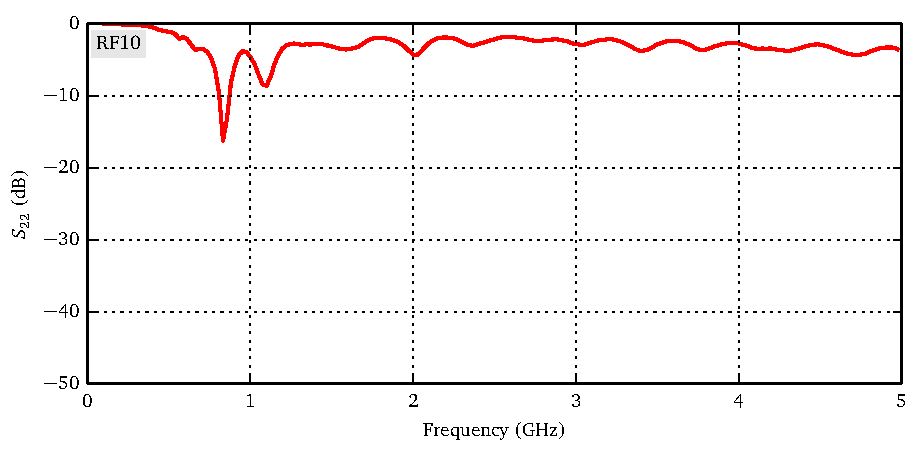
\includegraphics{figs/active/RF10-sParameters.pdf}
 \caption[Experimental $S_{22}$ trace of the RF10 fibre-antenna]
 		{Experimental $S_{22}$ trace for the RF10 fibre-antenna. 
 		The relatively background value of $\sim -4\,\unit{dB}$ indicates
 		that much of the power is reflected back from port 2 (the right-hand side of
 		the antenna, according to our specifications). Also, its single dip at $f\sim800\,\unit{MHz}$
 		is mostly useless for our purposes.}
 \label{fig:active.lcx.rf10sParameters}
\end{figure}

\begin{figure}
 \centering
 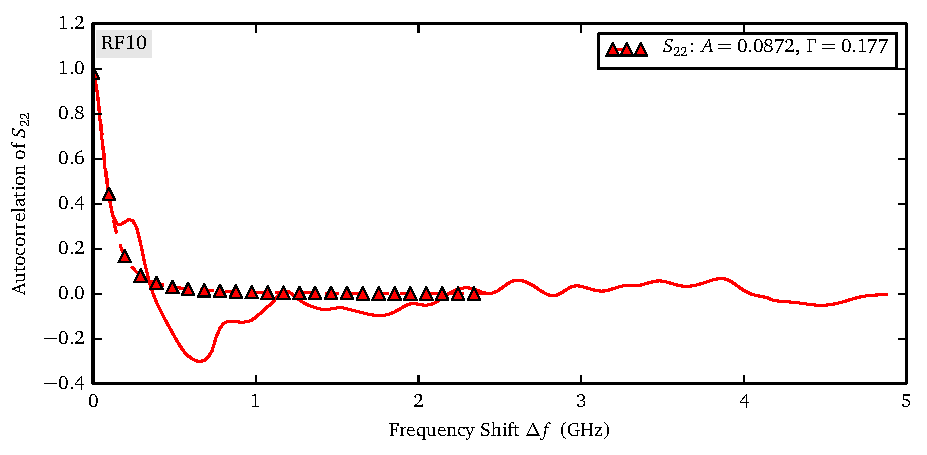
\includegraphics{figs/active/RF10-autoCorrelation.pdf}
 \caption[Autocorrelation of the experimental trace of $S_{22}$ for the RF10 fibre-antenna]
 		{Autocorrelation of the experimental trace of $S_{22}$ for the RF10 fibre-antenna.
 		The dotted line represents the Lorentzian fit. Despite relatively strong negative correlation around $800\,\unit{MHz}$,
 		it is almost zero over the whole interval, but does not fit the Lorentzian.}
 \label{fig:active.lcx.rf10autocorrelation}
\end{figure}

\paragraph{RF21}


\begin{figure}
 \centering
 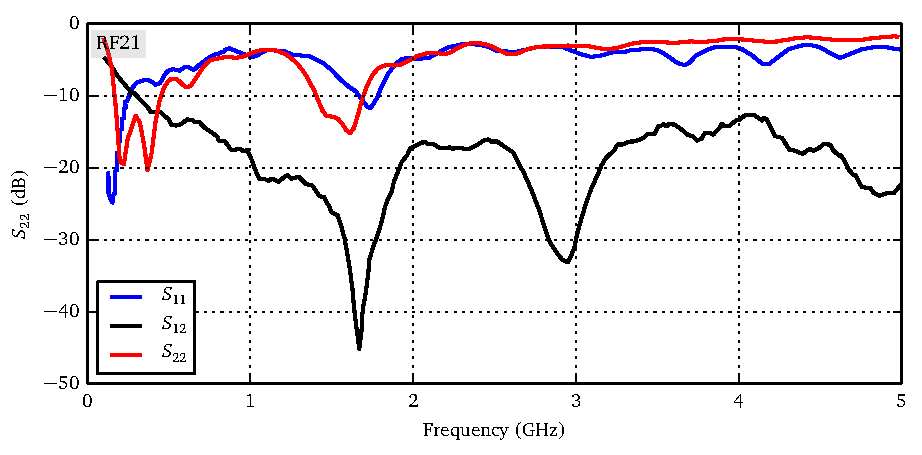
\includegraphics{figs/active/RF21-sParameters.pdf}
 \caption[Experimental $S_{22}$ trace for the RF21 fibre]
 		{Experimental $S_{22}$ trace for the RF21 fibre.}
 \label{fig:active.lcx.rf21sParameters}
\end{figure}

\begin{figure}
 \centering
 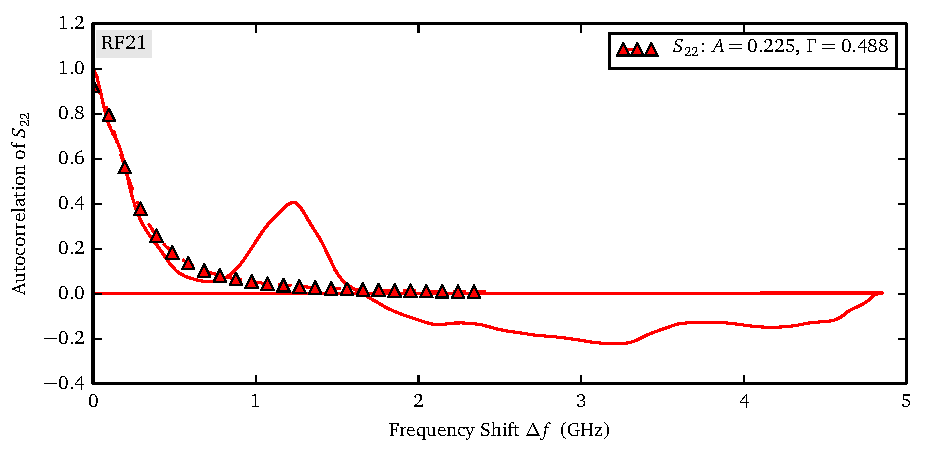
\includegraphics{figs/active/RF21-autoCorrelation.pdf}
 \caption[Autocorrelation of the experimental $S_{22}$ trace for the RF21 fibre-antenna]
 		{Autocorrelation of the experimental $S_{22}$ trace for the RF21 fibre-antenna.}
 \label{fig:active.lcx.rf21autocorrelation}
\end{figure}

\paragraph{RF27 and RF29}
As we can see from Table \ref{tab:antenna.rfxx-parameters}, these two antennae
are rather similar. It is thus not surprising that their $S$-parameters
show similar behaviour (compare Figures \ref{fig:active.lcx.rf27sParameters} and
\ref{fig:active.lcx.rf29sParameters}). Their small differences can be explained
away by the experimental variability of both the metal deposition and window
sizing protocols, as they have identical specifications.

Notice the quick decay of the autocorrelation function of the reflection 
coefficients, $S_{11}$ and $S_{22}$. If it were not for the hint of
regularity present in the autocorrelation function of $S_{12}$, 
it could be swiftly concluded that both antennae show chaotic scattering.
In any case, the lack of periodicity in the signals seems to indicate 
that the dip is not due to the geometry of the fibre-antenna. 

\begin{figure}
 \centering
 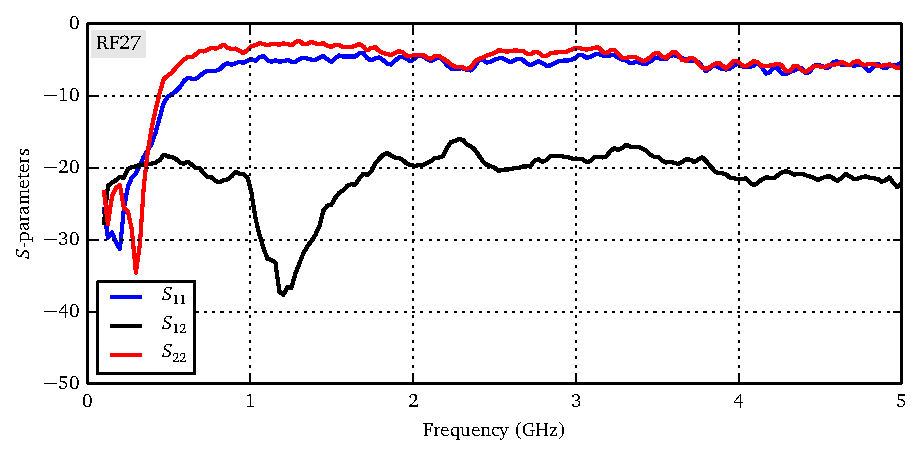
\includegraphics{figs/active/RF27-sParameters.pdf}
 \caption[Experimental $S$-parameter traces for the RF27 fibre-antenna]
 		{Experimental $S$-parameter traces for the RF27 fibre-antenna.}
 \label{fig:active.lcx.rf27sParameters}
\end{figure}

\begin{figure}
 \centering
 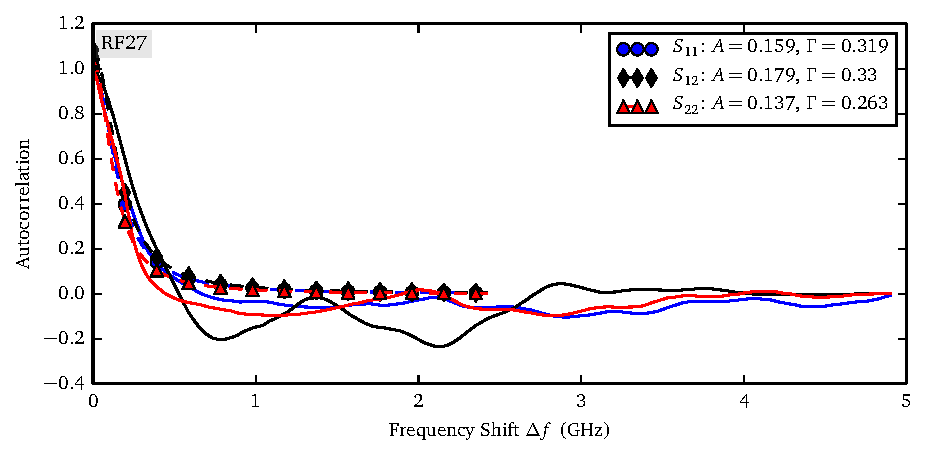
\includegraphics{figs/active/RF27-autoCorrelation.pdf}
 \caption[Autocorrelation of the experimental $S$-parameter traces for the RF27 fibre-antenna]
 		{Autocorrelation of the experimental $S$-parameter traces for the RF27 fibre-antenna.}
 \label{fig:active.lcx.rf27autocorrelation}
\end{figure}


\begin{figure}
 \centering
 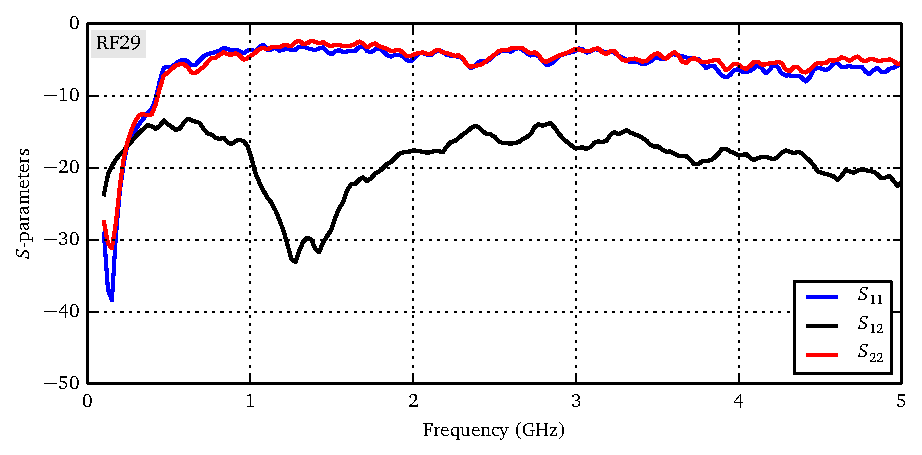
\includegraphics{figs/active/RF29-sParameters.pdf}
 \caption[Experimental $S$-parameter traces for the RF29 fibre-antenna]
 		{Experimental $S$-parameter traces for the RF29 fibre-antenna.}
 \label{fig:active.lcx.rf29sParameters}
\end{figure}

\begin{figure}
 \centering
 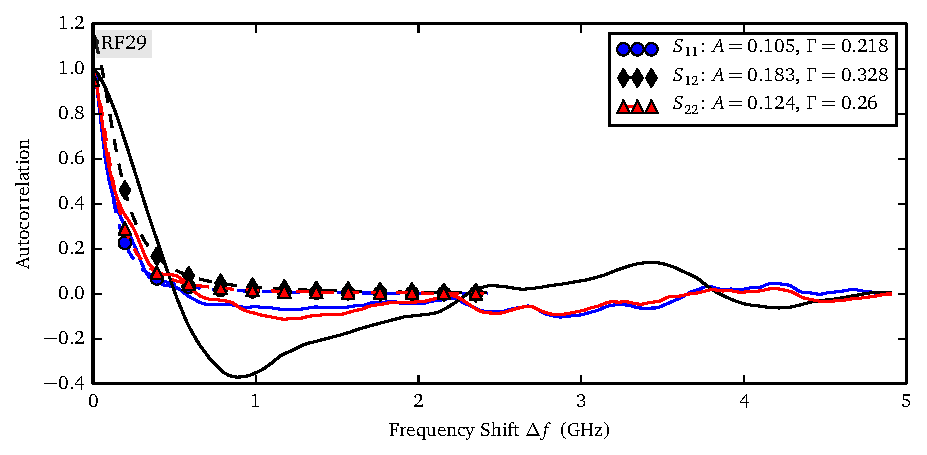
\includegraphics{figs/active/RF29-autoCorrelation.pdf}
 \caption[Autocorrelation of the experimental $S$-parameter traces for the RF29 fibre-antenna]
 		{Autocorrelation of the experimental $S$-parameter traces for the RF29 fibre-antenna.}
 \label{fig:active.lcx.rf29autocorrelation}
\end{figure}

\paragraph{RF33}
The RF33 fibre-antenna, the final antenna produced, is the most mature
one in terms of experimental protocol and is therefore most
worthy of study. 

\begin{figure}
 \centering
 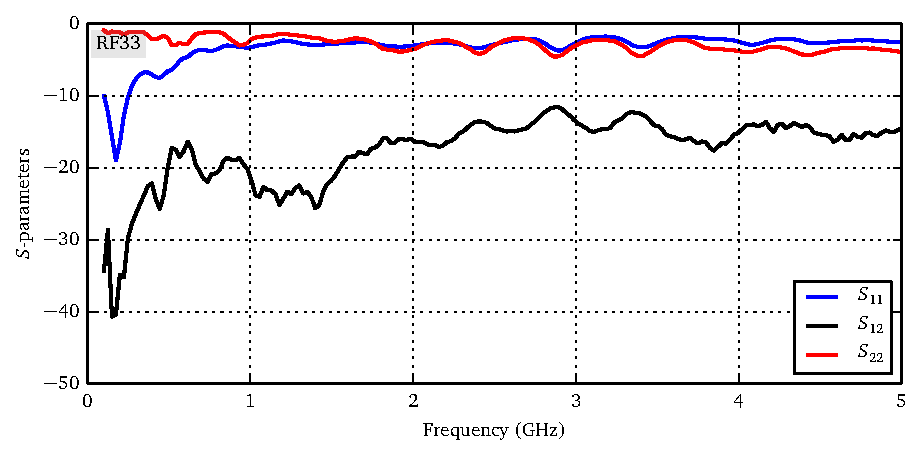
\includegraphics{figs/active/RF33-sParameters.pdf}
 \caption[Experimental $S$-parameter traces for the RF33 fibre-antenna]
 		{Experimental $S$-parameter traces for the RF33 fibre-antenna.}
 \label{fig:active.lcx.rf33sParameters}
\end{figure}

\begin{figure}
 \centering
 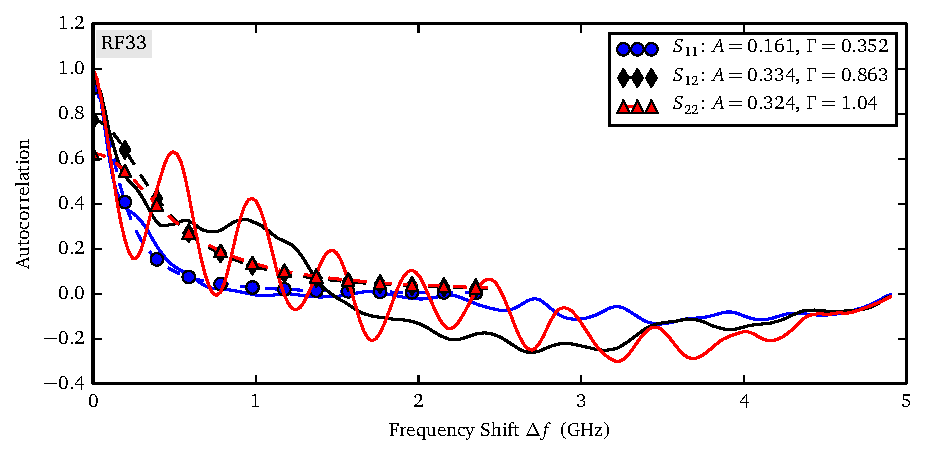
\includegraphics{figs/active/RF33-autoCorrelation.pdf}
 \caption[Autocorrelation of the experimental $S$-parameter traces for the RF33 fibre-antenna]
 		{Autocorrelation of the experimental $S$-parameter traces for the RF33 fibre-antenna.}
 \label{fig:active.lcx.rf33autocorrelation}
\end{figure}

\begin{figure}
 \centering
 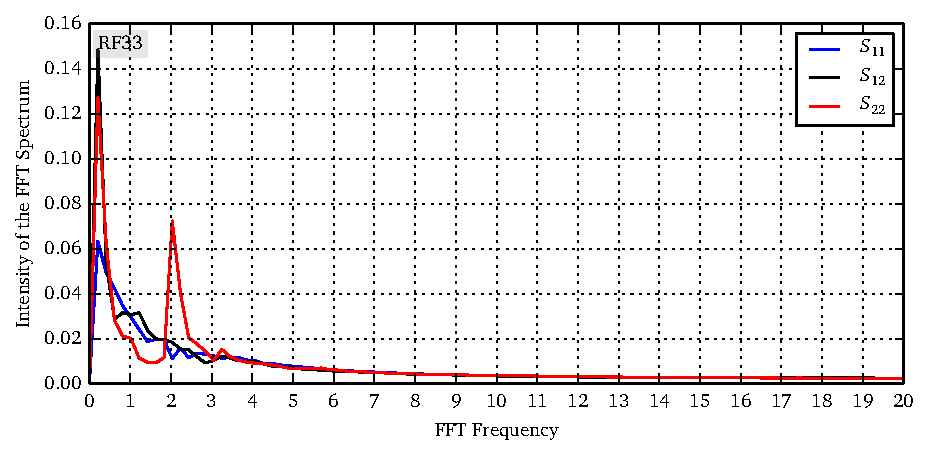
\includegraphics{figs/active/RF33-fft.pdf}
 \caption[FFT spectrum of the autocorrelation functions of the $S$-parameters of the RF33 fibre-antenna]
 		{FFT spectrum of the autocorrelation functions of the $S$-parameters of the RF33 fibre-antenna.}
 \label{fig:active.lcx.rf33fft}
\end{figure}


\subsection{Comparison with Simulation Results}

\subsubsection{Preliminary Results}
We first model the RF21 design. Its parameters are summarized in 
Table \ref{tab:antenna.rfxx-parameters}. 

\begin{figure}
 \centering
 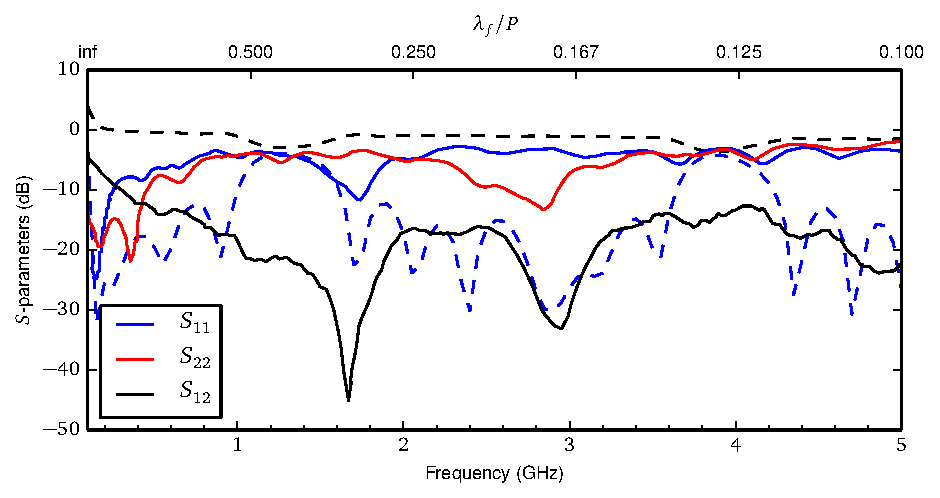
\includegraphics[width=\textwidth]{figs/active/sParametersRF21.pdf}
 \caption[$S$-parameters of the RF21 fibre design]
 		{$S$-parameters of the RF21 fibre design. The full lines represent
	  	the experimental data while the dotted lines represent the simulation data.
	  	The top $x$ axis shows the $S$-parameters as a function of the ratio of the 
	  	vacuum wavelength $\lambda_f$ over the period of the windows $P$.}
 \label{fig:antenna.sParameters}
\end{figure}

Notice the small thickness
of the silver layers (126 and 101 nm) compared to the other 
sizes involved. It takes a highly non-uniform mesh to model
these small relative sizes. Moreover, since the silver has a high
conductivity, it takes an even smaller mesh to model. Our first 
attempts at modeling this structure proved unsuccessful.

In the experimental data (\see Figure \ref{fig:antenna.sParameters}), 
we see deep dips in the transmission spectrum ($S_{12}$) at approximately
1.8 GHz and 3 GHz. There are corresponding dips in the reflection parameters,
$S_{11}$ and $S_{22}$, which leads us to believe that remaining power 
was radiated through the slots. The existence of two dips seems predicated on the asymmetry
of the fibre ($d_L\neq d_R$). 

We also notice that the simulation data does not in any way correlate
to the experimental data. This is probably due to the fact that, in the our
HFSS model, we had to put the thickness of the silvers layers to $2\,\unit{\mu m}$
instead of the values listed in Table \ref{tab:antenna.rfxx-parameters}. In 
this regime, the fibre-antenna behaves like an ordinary transmission line. 
However, as the mesher does not allow us to go under $2\,\unit{\mu m}$, we cannot
conclude that is really due to the thickness of the Ag layers, only suspect it.

In our previous simulations, it was clear that something was amiss:
there was no correlation between the simulation and
experimental data. AFM pictures (see Figure \ref{fig:antenna.AFM})  have suggested that the deposited
metal is in fact a mixture of silver and silver oxide. To evaluate
the effective conductivity of the mixture, we have used Bruggeman's model \cite{LAN1978}.
The model starts from a homogeneous medium, call it medium 1, 
of conductivity $\sigma_1$ and replaces spherical portions of this material 
by another one of conductivity $\sigma_2$. When this process is done, 
we are left with a inhomogeneous material with partial concentrations $\delta_i$
of each material. The effective conductivity $\sigma_e$ of the medium can be computed
using the relation (for an arbitrary number of materials)
  \begin{equation}
    \sum_i^n \delta_i \frac{\sigma_i-\sigma_e}{\sigma_i+(d-1)\sigma_e} =0 
  \end{equation}
where $\sum_i\delta_i=1$ and $d$ is the dimensionality of the system.
Solving for $\sigma_e$ in the case $n=2$ yields
  \begin{equation}
   (d-1)\sigma_e^2+\left[\left(d\delta_1-1\right)\sigma_1+\left(d\delta_2-1\right)\sigma_2\right]+\sigma_1\sigma_2=0.
  \end{equation}
The positive solution is, defining $q=\left(d\delta_1-1\right)\sigma_1+\left(d\delta_2-1\right)\sigma_2$
  \begin{equation}
   \label{eq:antenna:bruggeman}
   \sigma_e = \frac{1}{2d-2}\left[q+\sqrt{q^2+4(d-1)\sigma_1\sigma_2}\right].
  \end{equation}
  
\begin{figure}
 \centering
 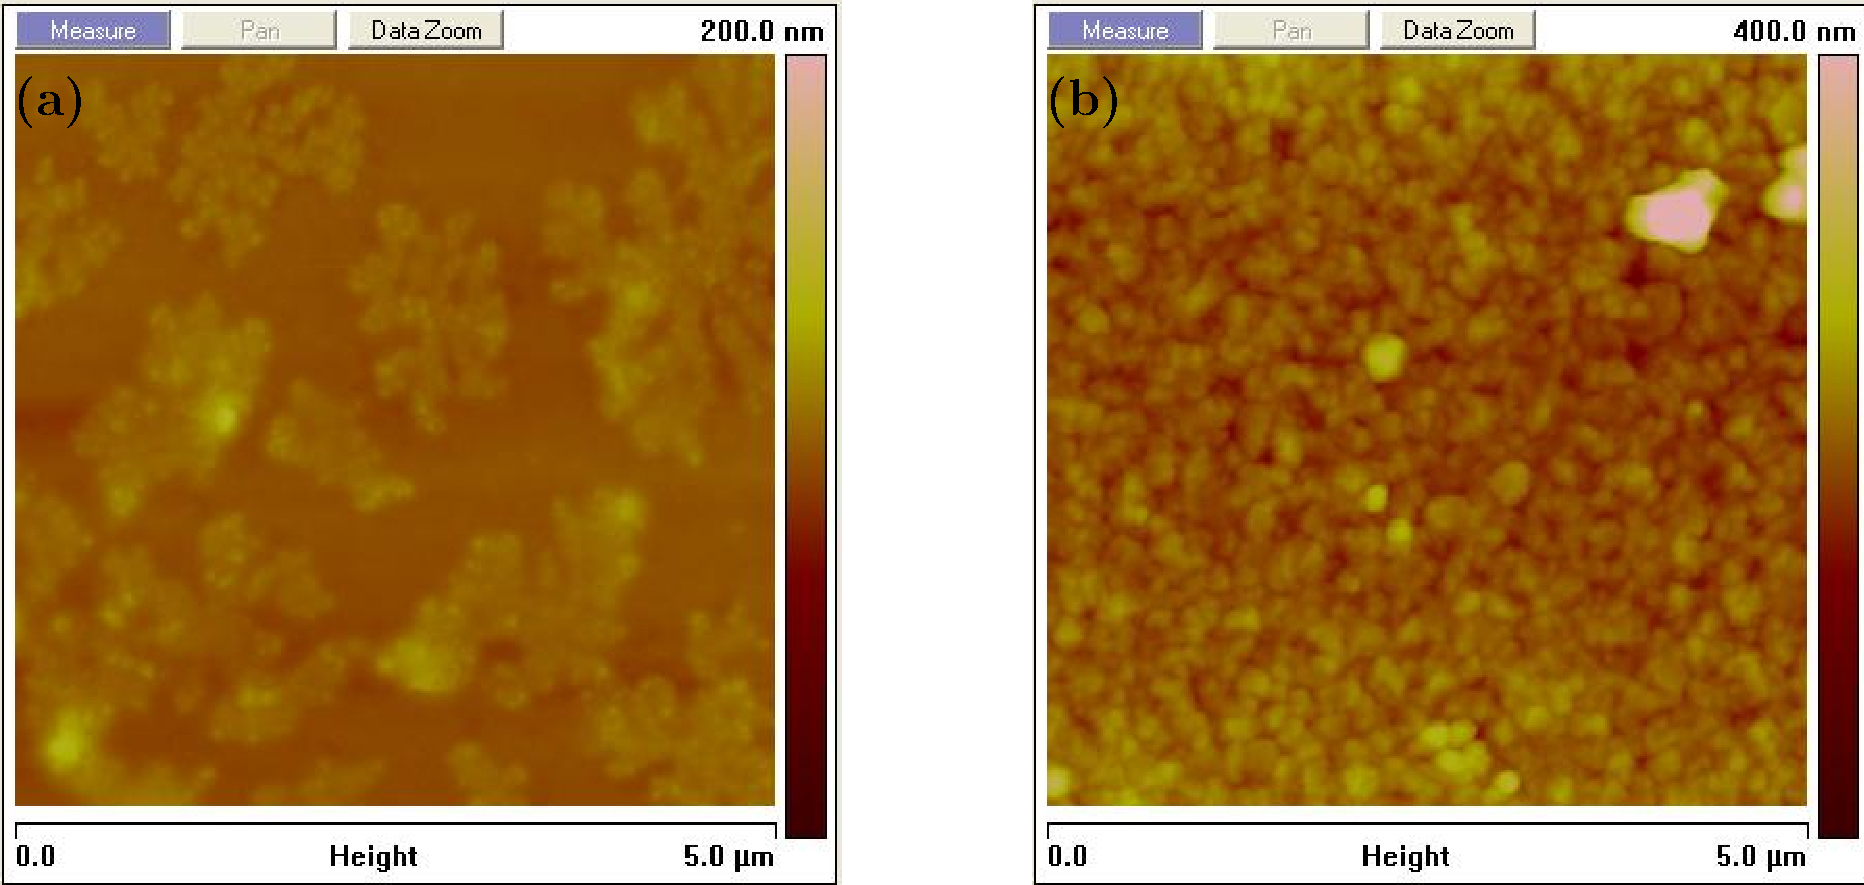
\includegraphics[width=0.8\textwidth]{figs/active/out/AFM.pdf}
 \caption[AFM pictures of silver deposited onto glass plates]
 		{AFM pictures of silver deposited onto glass plates. \textbf{(a)} Flakes of silver oxide seem to be forming onto the deposited
	  	silver layer. \textbf{(b)} Sample image showing the inhomogeneity of the
	  	silver layer.}
 \label{fig:antenna.AFM}
\end{figure}

Conductivity 
of thin metal films can be a function of their thicknesses. 
The Fuchs-Sondheimer model states
that
  \begin{equation}
      \sigma_F = \frac{\sigma_0}{1+\frac{3\lambda}{8d}\left(1-p\right)}
  \end{equation}
where $0\leq p\leq1$ is a specularity parameter that depends on the 
reflectivity of the electron gas, and $\lambda$ is the 
electron free mean path in the metal. This model states that conductivity
diminishes as the thickness of the metallic layer gets smaller.

In Figure \ref{fig:antenna.thicknessRatios}, we compare the 
thicknesses obtained via the bulk conductivity model (Bruggeman 
effective conductivity) and the Fuchs-Sondheimer model with 
effective conductivity for the RF33 fibre. Given that the AFM pictures
show surface inhomogeneity, we assume diffuse scattering in 
the FS model ($p=0$). We see that choosing a dimensionality 
of 3 or 2 does not significantly affect the thicknesses, but
we see a difference of about 20\% in the effective conductivities.

The most interesting thing, though, is that the FS
model predicts metallic layers that are 10\% to 80\% thicker 
than with the bulk conductivity model. 

\begin{table}
  \newcolumntype{d}{D{.}{.}{3}}
  \caption[Geometric and physical parameters of the \gls{lcx} antennae]
	  {Geometric and physical parameters of the \gls{lcx} antennae.
	  Units are repeated from column above if not indicated.}
 \begin{subtable}[t]{0.65\textwidth}
 \caption[Geometric parameters of the RF21/RF33 fibre designs]
	  {Geometric parameters of the fibre designs. 
	  The thicknesses of the layers are listed in order, stating
	  from the inner layer to the outer layer of the fibre-antenna.}
 \label{tab:antenna.rfxx-parameters}
 \begin{tabular*}{\textwidth}{l@{\extracolsep{\fill}}c@{\extracolsep{\fill}}d@{\extracolsep{\fill}}d@{\extracolsep{\fill}}d@{\extracolsep{\fill}}d}
  \hline\hline
  Quantity			& Unit			& \multicolumn{1}{c}{RF21} 	& \multicolumn{1}{c}{RF27\parnote{Measurements are approximate; values for the inner and outer resistances were lost. We assume they are identical to the RF29.}}	& \multicolumn{1}{c}{RF29}	& \multicolumn{1}{c}{RF33}	\\
  \hline
  $t_\text{vac}$	& $\unit{\mu m}$& 99.874					& 99.900					& 99.646			& 99.924			\\
  $t_\text{Ag1}$	& 				& 0.126						& 0.100						& 0.354				& 0.0766			\\
  $t_\text{Si}$		& 				& 273						& 273 						& 273				& 273				\\
  $t_\text{pyamide}$& 				& 24						& 24 						& 24 				& 24				\\
  $t_\text{Ag2}$	& 				& 0.101						& 0.100						& 0.306				& 0.030				\\
  $d_L$				& $\unit{mm}$	& 27						& 30						& 31				& 30.91				\\
  $d_R$				& 				& 55						& 55						& 55				& 54.72				\\
  $S_{z1}$\parnote{Each window has a different $S_z$ and $d_z$.}
					& 				& 32						& 34						& 33				& 34.36				\\
  $S_{z2}$			& 				& 32						& 34						& 34				& 34.06				\\
  $S_{z3}$			& 				& 32						& 34						& 33.5				& 33.87				\\
  $d_{z1}$			& 				& 28						& 28						& 29				& 27.44				\\
  $d_{z2}$			& 				& 28						& 28						& 28.5				& 28.36				\\
  $L$				& $\unit{cm}$	& 30.0						& 24.3						& 24.4				& 24.372			\\
  $\theta_w$		& $\unit{deg}$	& 180						& 180						& 180 				& 180				\\
  $R_\text{inner}$	& $\unit{\Omega}$& 60.0						& \multicolumn{1}{c}{---}	& 60				& 80.5				\\
  $R_\text{outer}$	&				& 20.0						& \multicolumn{1}{c}{---}	& 20				& 59.8				\\
  \hline\hline
 \end{tabular*}
 \begin{flushleft}
 \parnotes
 \end{flushleft}
 \end{subtable}\hfill
 \begin{subtable}[t]{0.3\textwidth}
  \begin{center}
 \caption{Physical parameters of the materials used in the fibre-antennae.}
 \label{tab:antenna.physicalParameters}
 \begin{tabular*}{\textwidth}{l@{\extracolsep{\fill}}c@{\extracolsep{\fill}}d}
  \hline\hline
  Quantity			& Unit			& \multicolumn{1}{c}{Value}		\\
  \hline
  $\epsilon_\text{Si}$		& --			& 3.77		\\
  $\epsilon_\text{pyamide}$	& --			& 3.50		\\
  $\sigma_\text{Ag0}$		& $\unitfrac{MS}{m}$	& 63.0		\\
  $\sigma_\text{AgO0}$		& 			&  6.79		\\
  $\lambda_\text{Ag}$		& $\unit{nm}$		& 40		\\
  \hline\hline
 \end{tabular*}
 \begin{flushleft}
 \parnotes
 \end{flushleft}
 \end{center}
 \end{subtable}
\end{table}

\begin{figure}
  \centering
  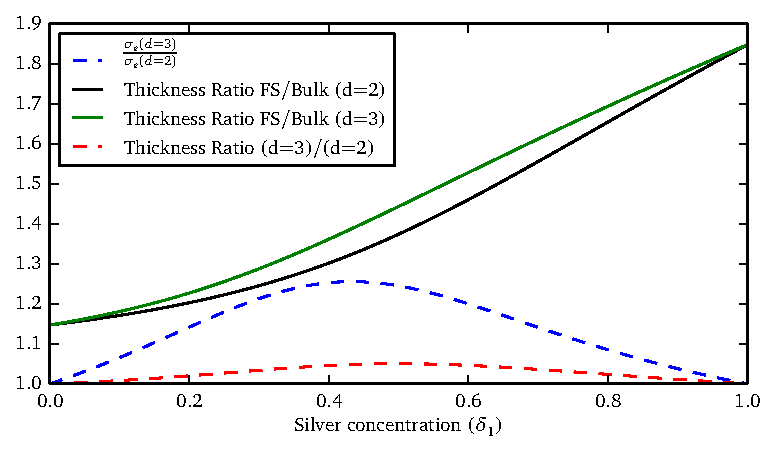
\includegraphics[width=0.9\textwidth]{figs/active/comparisonThickness.pdf}
  \caption[Thickness ratios as a function of the silver concentration]
	  {We show multiple ratios as a function of the silver concentration,
	  $\delta_1$. The blue line shows the ratio between the effective
	  conductivities for a choice of $d=2$ and $d=3$. The black and 
	  green lines show the ratio of the thickness predicted by using
	  the Fuchs-Sondheimer conductivity in Eq. \eqref{eq:antenna:thickGeneralEquations}
	  to the thickness predicted by using the bulk conductivity.
	  The red line shows the ratio of the green line to the black line.}
  \label{fig:antenna.thicknessRatios}
\end{figure}

We have simulated the RF21 fibre using Bruggeman's model
for the effective conductivity and with values
of $\delta_1\in\{0,1\}$ and $d=3$ in \eqref{eq:antenna:bruggeman}.
After obtaining the simulated $S_\text{11}$ parameter of the fibre,
we compared it to the experimentally obtained one using the Pearson
correlation coefficient. For two samples $\{X_i\}$ and 
$\{Y_i\}$, it is defined as
  \begin{equation}
    r = \frac{\sum_i^n\left(X_i-\left\langle X\right\rangle\right)\left(Y_i-\left\langle Y\right\rangle\right)}
	     {\sqrt{\sum_i^n\left(X_i-\left\langle X\right\rangle\right)^2}\sqrt{\sum_i^n\left(Y_i-\left\langle Y\right\rangle\right)^2}}.
  \end{equation}
From the definition, we see that the simultaneous linear transformations $X_i\rightarrow b+aX_i$ and $Y_i\rightarrow d+cY_1$
do not change the value of the Pearson coefficient. This means that even if the two samples
do not have the same normalization or are shifted by a constant amount, the correlation 
will stay the same. As such, the Pearson correlation measures the delegend(loc=1, prop={'size':6})
gree at which 
both samples are linearly related. 

Figure \ref{fig:antenna.sParameters} shows the experimental and simulated
$S_{11}$ parameter. At first look, it might seem like the general form 
of the curves are similar, but our quantitative analysis will show 
that that would be wrong. To make sure that our simulation data was not simply
shifted in frequency due to an small error in the geometry, we have
also calculated the correlation for a shifted dataset 
\footnote{To do so, we simply right-shifted the arrays containing
the simulation data and removed the data that fell outside the frequency range 
of the experimental data.}. This changes
the Pearson correlation because we must elide some of the experimental
and simulation data to do so. Figure \ref{fig:antenna.shiftCorrelation}
shows our results. We see that there are little to no correlation
between the simulation data and the experimental data with $r\in\{-0.04,0.05\}$. 

A possible source of error is the thickness of the silver layers. We will incorporate
the FS model in the next simulations and determine if it is
a factor. 

\begin{figure}
 \centering
 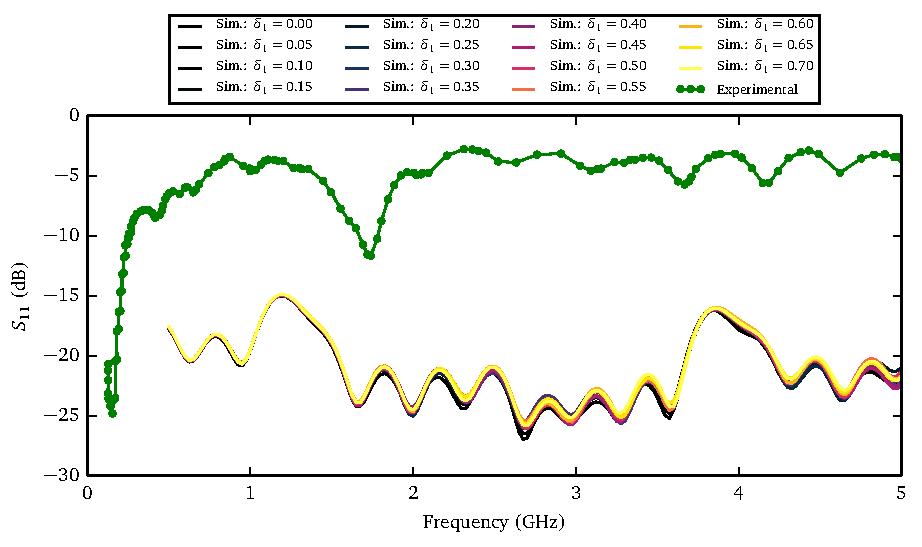
\includegraphics[width=0.8\textwidth]{figs/active/sParameters-concSweepS11.pdf}
 \caption[Experimental and simulated $S_{11}$ parameter for the RF21 fibre]
	 {Experimental and simulated $S_{11}$ parameter for the RF21 fibre.}
 \label{fig:antenna.sParameters}
\end{figure}

\begin{figure}
 \centering
 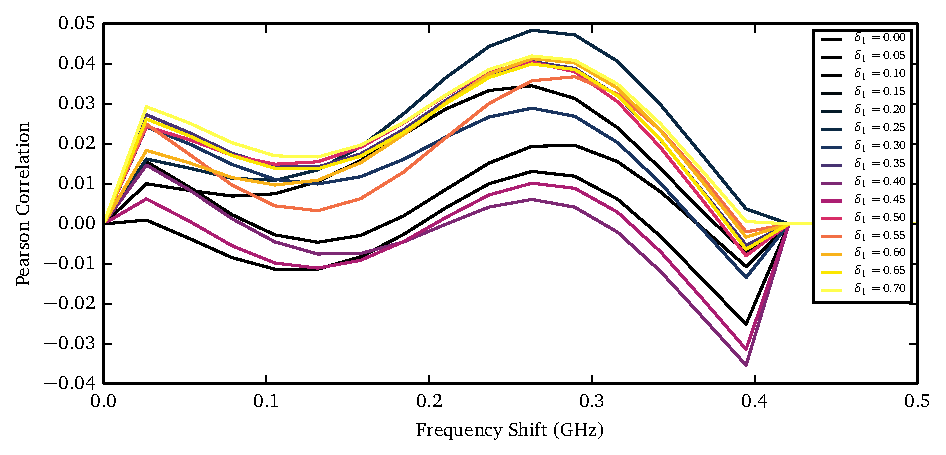
\includegraphics[width=0.8\textwidth]{figs/active/shiftCorrelationS11.pdf}
 \caption{Pearson correlation coefficient as a function of the frequency
	  shift of the data.}
 \label{fig:antenna.shiftCorrelation}
\end{figure}

We have also taken the Fourier transform of the experimental
and simulation data (for $\delta_1=0$). To our discontent, 
it seems that the datasets do not share periodic properties. 
Figure \ref{fig:antenna.fourierAnalysis} shows the intensity
of the FFT transform. To see if the periodic components corresponded
to particular lengths in the system, we converted the associated
wavelenghts to frequencies and plotted them as vertical lines in the figure. 
$f_1$ is the fundamental mode of infinite LCXF, namely
  \begin{equation}
   f_1 = \frac{c}{\left(S_z+d_z\right)\left(\sqrt{\epsilon_\text{Si}}+1\right)}.
  \end{equation}
The frequency associated with the optical and the actual lengths of the window
are
  \begin{align*}
   l_\text{opt}	&= \frac{c}{S_z\sqrt{\epsilon_\text{Si}}}	\\
   l_\text{phy}	&= \frac{c}{S_z}.
  \end{align*}

Nothing thus far seems to explain the periodic properties of the 
$S_{11}$ parameter of the experimental and simulation, although
the optical length of the windows seems to explain a single 
peak in the Fourier power spectrum. 

The author is not sure that is the proper method to
analyze the Fourier spectrum, however.

\begin{figure}
 \centering
 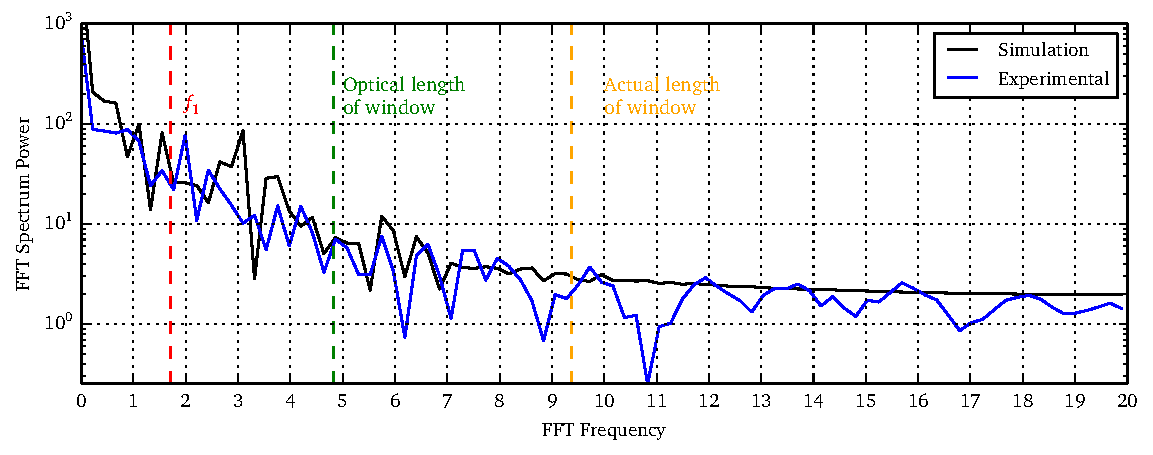
\includegraphics[width=0.8\textwidth]{figs/active/fourierAnalysisS11.pdf}
 \caption[Fourier Power Spectrum]
	  {Absolute value of the Fourier transform of the $S_{11}$ parameter.
	  The red lines denote the frequencies associated with certain lengths
	  in the RF21 fibre design.}
 \label{fig:antenna.fourierAnalysis}
\end{figure}



% \section{Antenna Propagation}
% 
% \todo[inline]{Describe goal of project; advantages of using fibers
% 	      over patch antennae...}
% 	      
% \subsection{Antenna Theory Primer}
% \todo[inline]{Basic definitions of directivity, gain...}
% \todo[inline]{Stratton solution}
% 
% \subsection{Designs}
% 
% \todo[inline]{Feasability of design via dipole antenna. Analytical solution
% 	      of dipole antenna. Issue with thin silver shells.}
% 
% \todo[inline]{Theory of infinite LCXs as guide for finite LCX. Discuss in more
% 	      detail about the thin silver shells (methods used to model them,
% 	      non-agreement with experimental data and its probable causes).
% 	      Discuss Bruggemann's model and Fuchs-Sondheimer methods.}